
\documentclass[10pt,letterpaper]{article}
\usepackage[utf8]{inputenc}\usepackage[T1]{fontenc}\usepackage{lmodern}
\usepackage[letterpaper,top=1.2cm,bottom=1.15cm,left=1.3cm,right=1.3cm,headheight=14pt]{geometry}
\usepackage{graphicx,xcolor,booktabs,tabularx,array,amsmath,amssymb,hyperref}
\newcolumntype{C}{>{\centering\arraybackslash}X}
\definecolor{navy}{HTML}{102A43}\definecolor{blue}{HTML}{184E77}\definecolor{teal}{HTML}{2A9D8F}\definecolor{gold}{HTML}{E9B949}\definecolor{ink}{HTML}{172033}\definecolor{pale}{HTML}{EDF5FB}\definecolor{mint}{HTML}{E8F6F3}
\hypersetup{colorlinks=true,urlcolor=teal,linkcolor=blue,pdftitle={Laboratorio 5 - Reto Babel optimizado},pdfauthor={Barillas, Gualim y Ocaña}}
\setlength{\parindent}{0pt}\setlength{\parskip}{3pt}\renewcommand{\arraystretch}{1.13}
\newcommand{\labsection}[1]{\vspace{1mm}{\Large\bfseries\color{navy}#1}\par\vspace{1mm}{\color{teal}\hrule height .7pt}\vspace{2mm}}
\newcommand{\labsub}[1]{\vspace{1.5mm}{\normalsize\bfseries\color{blue}#1}\par}
\newenvironment{info}[1][]{\par\smallskip\noindent\begin{minipage}{.96\linewidth}\color{ink}\textbf{\color{teal}#1}\par\smallskip}{\end{minipage}\par\smallskip}
\makeatletter\def\ps@lab{\def\@oddhead{\small\color{navy}\textbf{Laboratorio 5 · Reto Babel}\hfil\color{teal}Barillas · Gualim · Ocaña}\def\@evenhead{\@oddhead}\def\@oddfoot{\hfil\small\color{blue}\thepage\ / 7\hfil}\def\@evenfoot{\@oddfoot}}\makeatother\pagestyle{lab}
\begin{document}
\thispagestyle{empty}\pagecolor{navy}\color{white}\vspace*{.5cm}
{\small\bfseries DEEP LEARNING \quad LABORATORIO 05 \quad OPTIMIZACIÓN POST-EDA}\par\vspace{1.3cm}
{\fontsize{30}{34}\selectfont\bfseries Reto Babel:\par del diagnóstico estructural al 100\%}\par\vspace{.4cm}
{\Large Transformer compacto, selección multisemilla y prueba secreta congelada}\par\vspace{1cm}
\colorbox{white}{\begin{minipage}{.92\linewidth}\color{ink}\small
\begin{tabularx}{\linewidth}{>{\bfseries\color{blue}}l X >{\bfseries\color{blue}}l X}
Institución & Universidad del Valle de Guatemala & Curso & Deep Learning y Sistemas Inteligentes\\
Docente & Kevin Recinos & Integrante A & Pablo Daniel Barillas Moreno · 22193\\
Modalidad & Grupo de tres & Integrante B & Cindy Mishelle Gualim Pérez · 221226\\
Entrega & 6 de septiembre de 2026 & Integrante C & Gadiel Ocaña · 231270
\end{tabularx}\end{minipage}}\par\vfill
\colorbox{teal}{\begin{minipage}{.92\linewidth}\color{white}\small\textbf{Resultado.} El modelo final alcanzó 240/240 frases oficiales, 1,519/1,519 tokens y 10/10 secretos coherentes, conservando 98,810 parámetros. La selección se realizó sin usar los secretos.\end{minipage}}\par\vspace{.7cm}
\begin{center}\color{gold}\Large 94.17\% $\rightarrow$ 100\% de frases exactas\end{center}
\newpage\nopagecolor\color{ink}

\labsection{Investigación: por qué atención, posición y máscaras}
\small
Una RNN encadena $h_t$ con $h_{t-1}$, limitando el paralelismo. El Transformer sustituye recurrencia por atención y permite relacionar posiciones directamente. En traducción, el encoder contextualiza la frase completa; el decoder usa self-attention causal y atención cruzada para producir el objetivo condicionado por la memoria fuente.
\[
\operatorname{Attention}(Q,K,V)=\operatorname{softmax}\left(\frac{QK^\top}{\sqrt{d_k}}+M\right)V.
\]
La máscara $M$ bloquea padding y futuro. Sin información posicional, la atención ve contenido pero no sabe qué elemento apareció primero. La codificación sinusoidal suma coordenadas al embedding y permite distinguir roles dependientes del orden.
\labsub{Arquitectura preservada}
\begin{center}\begin{tabularx}{.94\linewidth}{X C C C C C}
\toprule & $d_{model}$ & Cabezas & Capas E/D & $d_{ff}$ & Parámetros\\\midrule
Baseline y ganador & 48 & 4 & 2/2 & 96 & 98,810\\\bottomrule
\end{tabularx}\end{center}
\begin{info}[Idea central]
El objetivo no fue maximizar capacidad, sino corregir el patrón de error con el menor modelo. La red final sigue usando \texttt{nn.Transformer}, máscaras booleanas, teacher forcing, clipping de gradiente y greedy decoding.
\end{info}
\labsub{Ventaja y costo}
Self-attention procesa posiciones en paralelo y reduce la distancia entre tokens, pero construye relaciones cuadráticas en el largo. Como Babel usa secuencias de 5--7 tokens, el costo es pequeño; la ventaja principal es estructural y experimental.
\labsub{Flujo tensorial implementado}
\begin{tabularx}{\linewidth}{>{\bfseries\color{blue}}l X l}
\toprule Etapa & Operación & Forma principal\\\midrule
Fuente & Tokenización, \texttt{<SOS>/<EOS>}, padding y embedding posicional & $[B,S,d]$\\
Encoder & Self-attention bidireccional sobre tokens no padding & $[B,S,d]$\\
Objetivo & Desplazamiento: entrada $y_{<t}$ y etiqueta $y_t$ & $[B,T]$\\
Decoder & Máscara causal, self-attention y atención cruzada & $[B,T,d]$\\
Salida & Proyección al vocabulario y \texttt{CrossEntropyLoss} & $[B,T,|V|]$\\\bottomrule
\end{tabularx}
\labsub{Teacher forcing y controles}
Durante entrenamiento el decoder recibe el prefijo verdadero, de modo que
$\mathcal{L}=-\sum_t\log p_\theta(y_t\mid y_{<t},x)$; en inferencia recibe sus propias predicciones. La máscara triangular impide consultar $y_{>t}$ y la máscara de padding evita atender relleno. Los \texttt{asserts} verifican forma, diagonal visible, futuro bloqueado y conteo de parámetros.
\vfill{\footnotesize Fuente: Vaswani et al. (2017), secciones 1, 3 y 4; documentación oficial de PyTorch.}
\newpage

\labsection{Datos y EDA: de la señal al diagnóstico}
\small
\begin{tabularx}{\linewidth}{X r r X}\toprule Indicador & Train & Validación & Lectura\\\midrule
Frases únicas & 1,200 & 240 & Sin duplicados internos\\
Traslape literal & \multicolumn{2}{c}{0} & Sin memorización de frases\\
OOV & --- & 0 & Vocabulario completamente cubierto\\
Longitud & 5--7 & 5--7 & Distribución comparable\\
Negación & 49.25\% & 47.92\% & Estable\\
Mismo determinante & 43.42\% & 48.33\% & Principal ambigüedad\\\bottomrule\end{tabularx}
\labsub{Hallazgo nuevo de cobertura}
Las 56 parejas ordenadas sujeto--objeto aparecen en entrenamiento, con 13--31 ejemplos cada una. Sin embargo, ninguna de las 240 composiciones completas de validación repite exactamente sujeto, objeto, verbo, adjetivo y negación. La tarea exige recombinar factores conocidos.
\labsub{Patrón de error histórico}
El baseline falló 14 frases y 28 tokens. Los ejemplos exportados preservaban verbo, negación y adjetivo, pero invertían sujeto y objeto cuando ambos compartían artículo. Por tanto, ampliar vocabulario, beam search o más embeddings no atacaba el problema.
\begin{info}[Decisión derivada del EDA]
Extender entrenamiento, suavizar etiquetas y aumentar la exposición de estructuras simétricas; mantener arquitectura y datos intactos.
\end{info}
\begin{center}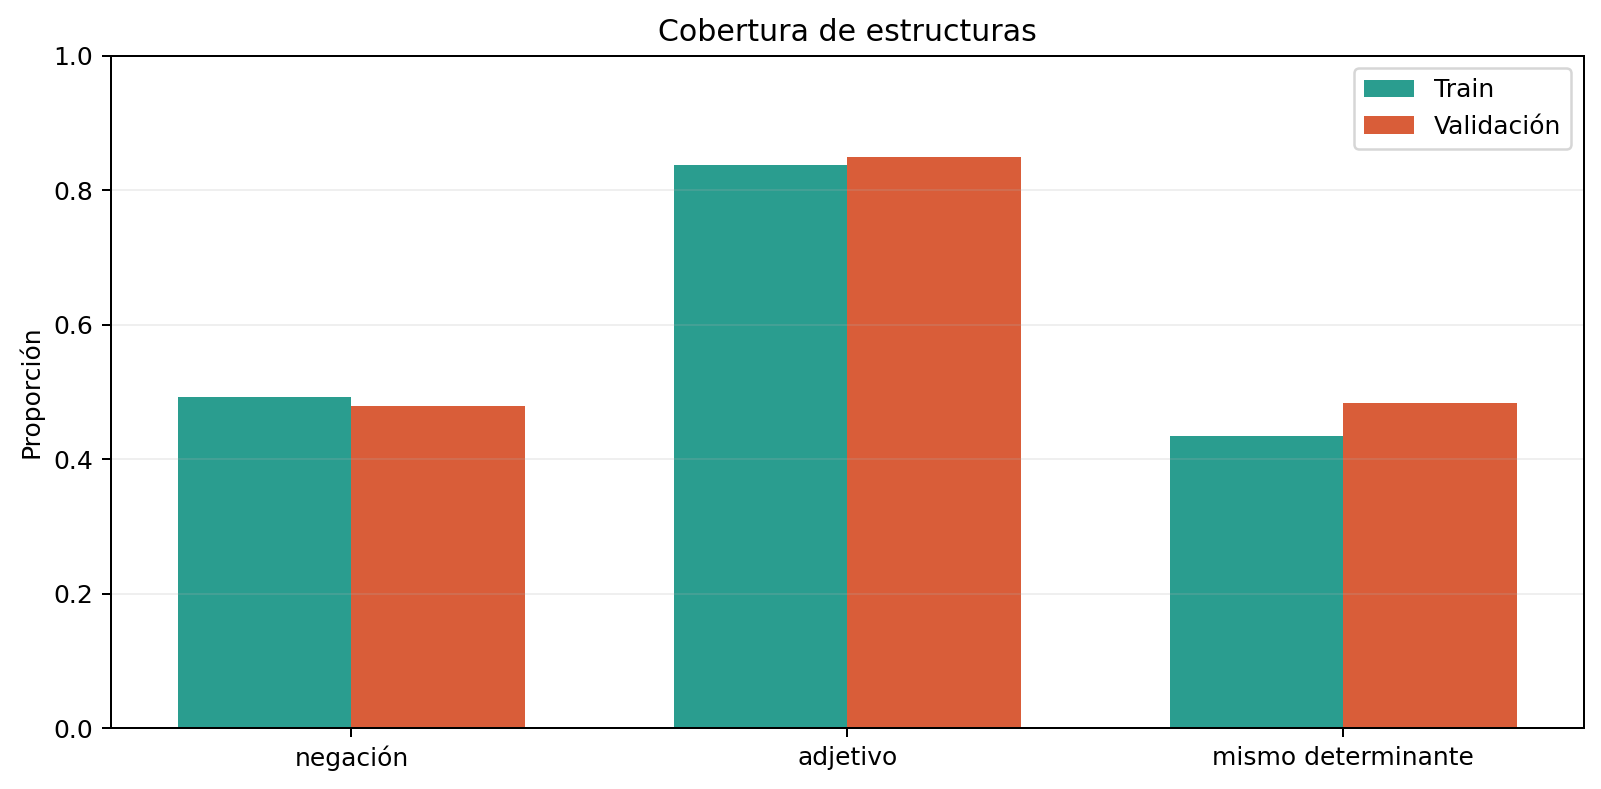
\includegraphics[width=.83\linewidth]{../evidencia/figuras/eda_estructuras.png}\end{center}
\labsub{Hipótesis convertidas en experimentos}
\begin{tabularx}{\linewidth}{X X X}
\toprule Evidencia & Hipótesis & Prueba controlada\\\midrule
Mejor pérdida en la época 22 & Subentrenamiento & 50 épocas con parada temprana interna\\
Errores de intercambio de roles & Exposición insuficiente a simetrías & Muestreo con pesos 1.5, 2.0 y 3.0\\
Cero OOV y cobertura completa & No falta vocabulario & Arquitectura y embeddings sin cambios\\
Composiciones oficiales nuevas & Se requiere recombinación & Exactitud de frase y análisis por subgrupo\\\bottomrule
\end{tabularx}
La asociación entre estructura y error se calculó sin alterar etiquetas. La validación oficial se reservó para la comparación posterior al congelamiento; esto separa diagnóstico, selección interna y reporte final.
\newpage

\labsection{Protocolo de optimización sin fuga}
\footnotesize
Las 1,200 frases se dividieron 960/240 estratificando negación, adjetivo, determinantes y longitud. La selección usó frases exactas, luego tokens y finalmente menos parámetros. Los secretos permanecieron ocultos. Los dos finalistas se repitieron con semillas 17, 42 y 73.
\labsub{Primera búsqueda}
\begin{tabularx}{\linewidth}{X C C C}\toprule Experimento & Frases & Tokens & Parámetros\\\midrule
Entrenamiento extendido & 86.67\% & 95.79\% & 98,810\\
Label smoothing 0.05 & 90.00\% & 96.84\% & 98,810\\
Muestreo estructural 2.0 & 93.33\% & 97.89\% & 98,810\\
$d_{model}=56$ & 75.00\% & 88.55\% & 133,194\\
$d_{model}=64$ & 62.92\% & 82.88\% & 172,698\\
Pre-LN + GELU & 84.17\% & 95.00\% & 98,810\\\bottomrule\end{tabularx}
\labsub{Refinamiento enfocado}
Se aisló Adam + $\varepsilon=0.05$ + pesos difíciles 1.5, 2.0 y 3.0. Peso 2.0 obtuvo 100\% con semilla 42 pero 85.42\% con semilla 73. Peso 3.0 promedió 96.53\% y fue el ganador robusto. La mediana de sus mejores épocas fijó 48 épocas finales.
\begin{center}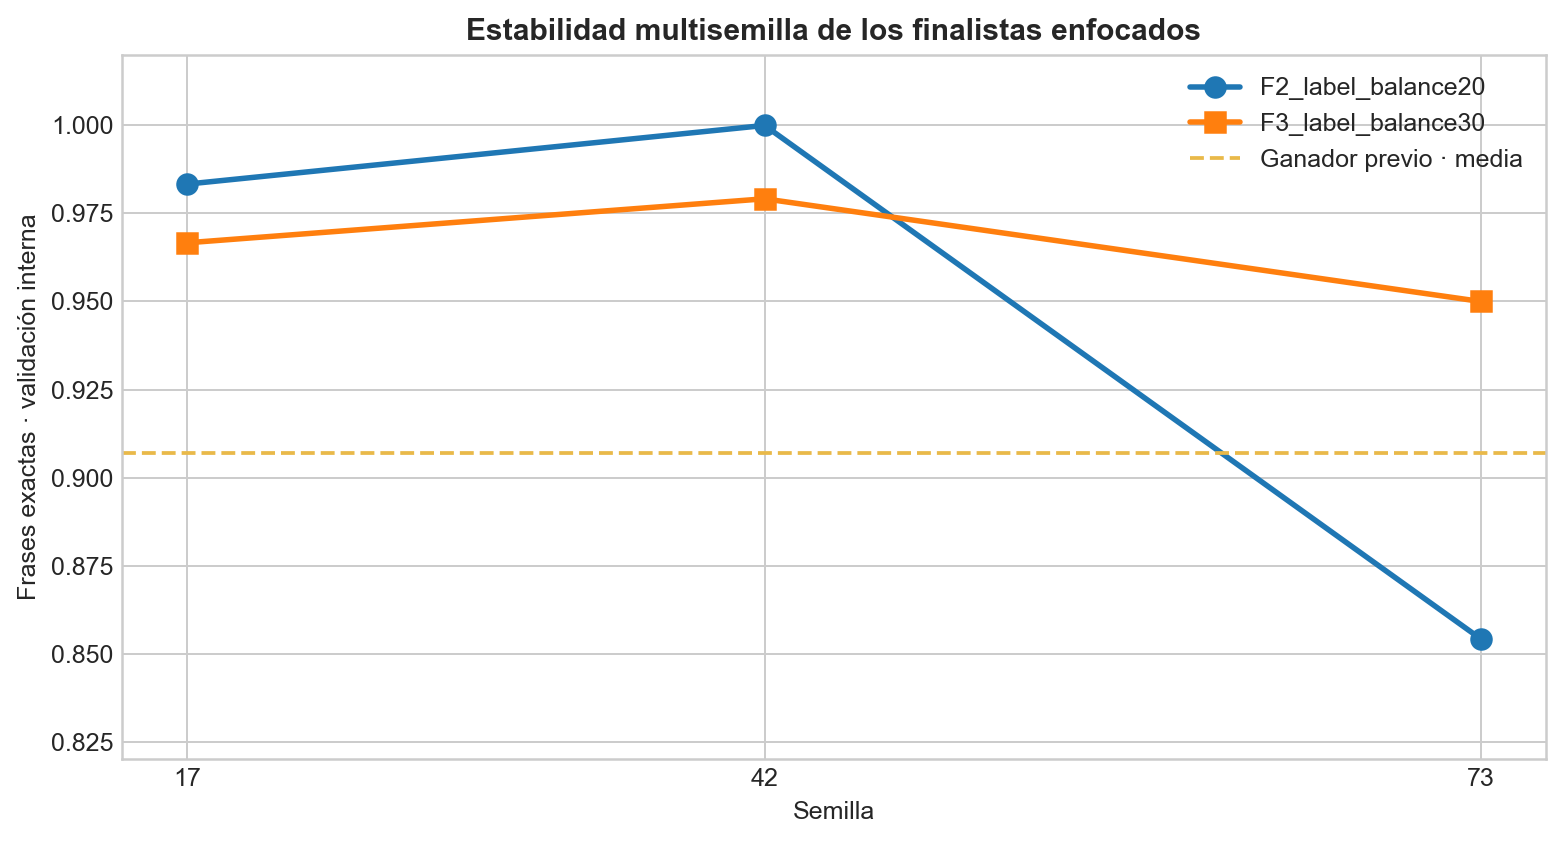
\includegraphics[width=.72\linewidth]{../evidencia/figuras/estabilidad_multisemilla.png}\end{center}
\labsub{Salvaguardas de selección}
\begin{tabularx}{\linewidth}{l X}
\toprule Control & Aplicación\\\midrule
Estratificación & Negación, adjetivo, igualdad de determinante y longitud.\\
Orden de métricas & Frases exactas $\rightarrow$ tokens $\rightarrow$ menor cantidad de parámetros.\\
Robustez & Tres semillas para finalistas; se rechazó el pico aislado de peso 2.0.\\
Prueba secreta & Acceso únicamente después de fijar configuración, épocas y semilla.\\
Trazabilidad & JSON con configuraciones, predicciones, subgrupos y hashes SHA-256.\\\bottomrule
\end{tabularx}
\begin{info}[Configuración congelada]
Adam, $lr=0.002$, dropout 0.1, label smoothing 0.05, peso estructural 3.0, 48 épocas y greedy. Beam 3/5 no cambió ninguna traducción y fue descartado.
\end{info}
\newpage

\labsection{Resultado cuantitativo final}
\small
\begin{center}\begin{tabularx}{.9\linewidth}{X C C C}\toprule Configuración & Tokens & Frases & Parámetros\\\midrule
Baseline histórico & 98.16\% & 94.17\% (226/240) & 98,810\\
Optimizado post-EDA & \textbf{100\%} & \textbf{100\% (240/240)} & 98,810\\
Sin posición & 74.72\% & 47.50\% (114/240) & 98,810\\\bottomrule\end{tabularx}\end{center}
\begin{center}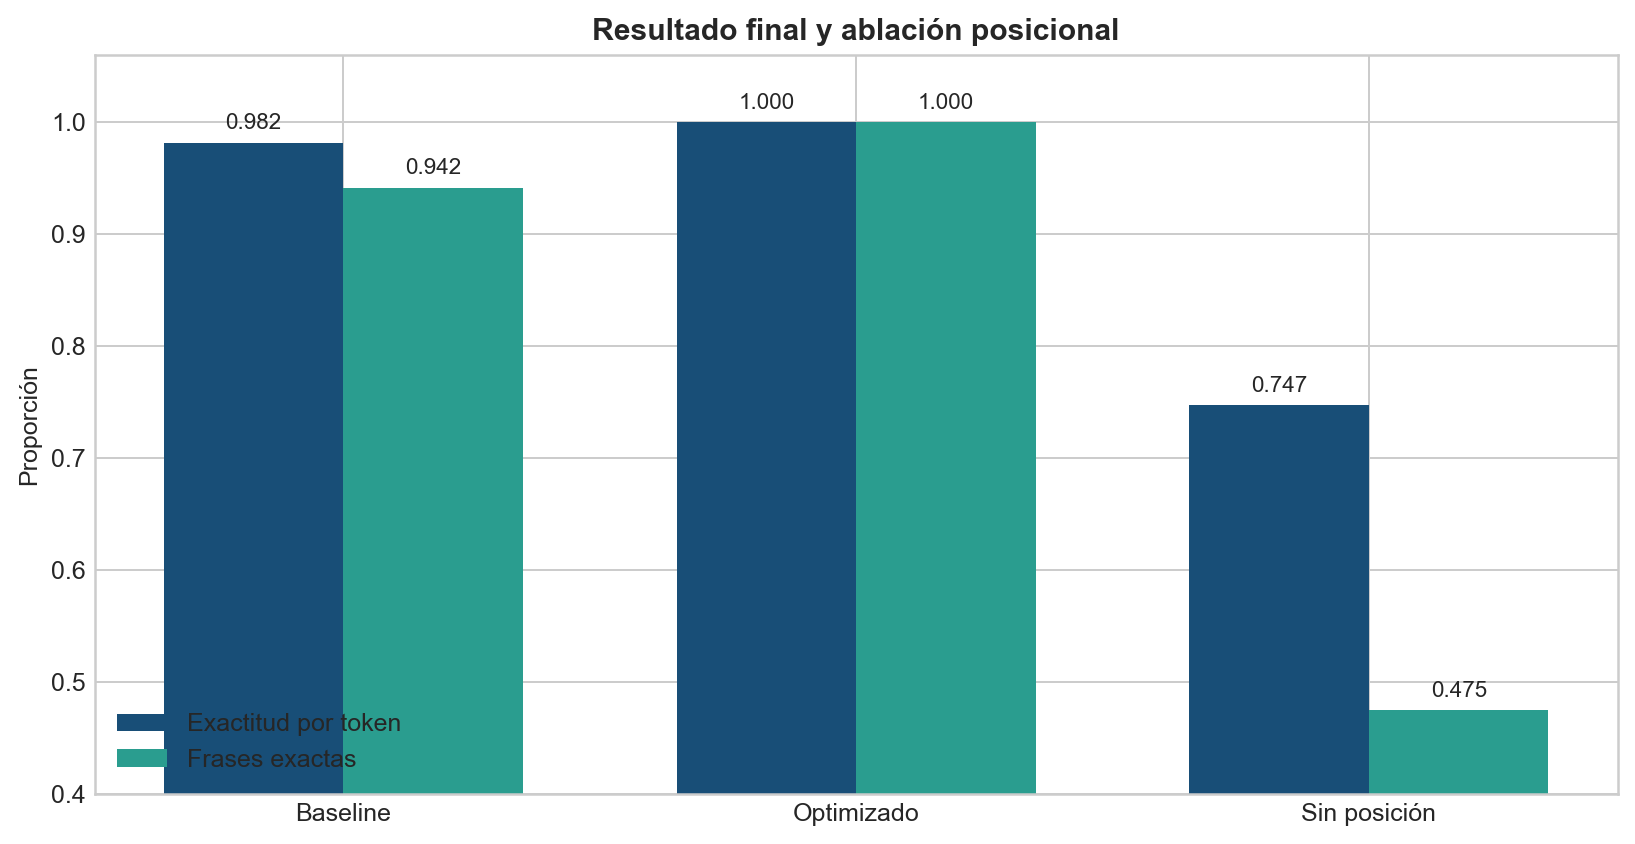
\includegraphics[width=.9\linewidth]{../evidencia/figuras/resultado_final_optimizacion.png}\end{center}
\labsub{Magnitud}
La mejora es de \textbf{+1.84 pp por token} y \textbf{+5.83 pp por frase}. Se corrigieron los 14 errores, una reducción relativa del 100\%, sin agregar parámetros ni complejidad de decoding.
\labsub{Subgrupos}
Todos los subgrupos quedaron en 100\%: mismo/diferente determinante, con/sin negación, con/sin adjetivo y longitudes 5, 6 y 7. Esto confirma que la intervención corrigió específicamente el residuo estructural.
\begin{center}\begin{tabularx}{.94\linewidth}{X r r X r r}
\toprule Subgrupo & Bien & Total & Subgrupo & Bien & Total\\\midrule
Mismo determinante & 116 & 116 & Determinante diferente & 124 & 124\\
Con negación & 115 & 115 & Sin negación & 125 & 125\\
Con adjetivo & 204 & 204 & Sin adjetivo & 36 & 36\\
Longitud 5 & 18 & 18 & Longitud 6/7 & 222 & 222\\\bottomrule
\end{tabularx}\end{center}
\labsub{Lectura pareada del error}
El baseline acertaba casi todos los tokens porque una frase con dos roles intercambiados suma solo dos errores; sin embargo, la frase completa queda semánticamente equivocada. Por eso 98.16\% por token coexistía con 14 traducciones incorrectas. La métrica de frase exacta fue el criterio primario y la exactitud por token quedó como diagnóstico secundario.
\begin{info}[Lectura correcta]
No se compara pérdida bruta con el baseline porque label smoothing cambia el objetivo. La evidencia comparable son exactitud, frases, errores, parámetros y evaluación pareada sobre los mismos 240 ejemplos.
\end{info}
\newpage

\labsection{Ablación y prueba secreta}
\footnotesize
\labsub{Ablación posicional}
Con datos, semilla, arquitectura, sampler, pérdida y 48 épocas constantes, retirar posición reduce frases de 100\% a 47.50\% y tokens de 100\% a 74.72\%. La diferencia causal es 52.50 pp por frase.
La caída es coherente con la hipótesis: sin coordenadas posicionales, self-attention puede reconocer palabras pero no distinguir de forma confiable quién ejecuta la acción y quién la recibe. La ablación modifica una sola variable y convierte esa afirmación conceptual en evidencia experimental.
\labsub{Diez frases secretas}
Se evaluaron después de congelar el modelo. La referencia se obtuvo del diccionario y reglas explícitas, no de un traductor externo.
\par\medskip\noindent
\begin{tabularx}{\linewidth}{r >{\ttfamily\raggedright\arraybackslash}X}
\toprule \# & Secreto $\rightarrow$ traducción generada\\\midrule
1 & moro seza fefo povo mefi zita $\rightarrow$ \rmfamily la maestra encuentra el músico grande\\
2 & fefo mefi moro somi bane $\rightarrow$ \rmfamily el músico mira la niña\\
3 & fefo rino fefo posi zizi gope riga $\rightarrow$ \rmfamily el perro no busca el jardinero feliz\\
4 & moro sesi moro mapa gope riga $\rightarrow$ \rmfamily la gata no busca la médica\\
5 & fefo zizi fefo posi gero gope riga $\rightarrow$ \rmfamily el jardinero no busca el niño feliz\\
6 & fefo zizi moro povo seza rizo $\rightarrow$ \rmfamily el jardinero cuida la maestra grande\\
7 & moro sesi moro sena seza pefe riga $\rightarrow$ \rmfamily la gata no lleva la maestra verde\\
8 & moro somi fefo gero gope riga $\rightarrow$ \rmfamily la niña no busca el niño\\
9 & moro sesi moro sena mapa gope riga $\rightarrow$ \rmfamily la gata no busca la médica verde\\
10 & fefo gero fefo ragi rino nava $\rightarrow$ \rmfamily el niño lee el perro joven\\\bottomrule
\end{tabularx}
\begin{info}[Resultado secreto]
10/10 traducciones coincidieron con las referencias. Esto es evidencia adicional posterior a selección; no reemplaza una cohorte futura independiente del profesor.
\end{info}
\labsub{Cobertura estructural del reto secreto}
\begin{tabularx}{\linewidth}{X r X r X r}
\toprule Rasgo & Casos & Rasgo & Casos & Rasgo & Casos\\\midrule
Con negación & 5/10 & Con adjetivo & 7/10 & Mismo determinante & 6/10\\
Sin negación & 5/10 & Sin adjetivo & 3/10 & Determinante distinto & 4/10\\\bottomrule
\end{tabularx}
La prueba no se limita a una plantilla: combina afirmación y negación, modificadores opcionales y pares nominales potencialmente ambiguos. Las diez salidas preservan concordancia, posición del adjetivo y alcance de \emph{no}.
\labsub{Controles de calidad de la decodificación}
\begin{itemize}
\item Cada secuencia inicia con \texttt{<SOS>}, termina al producir \texttt{<EOS>} y nunca expone \texttt{<PAD>} al texto final.
\item La predicción se genera token por token; no se copia la referencia ni se usa un traductor externo.
\item Beam widths 3 y 5 reprodujeron exactamente las salidas greedy, por lo que se conservó el método más simple.
\item La lista secreta se incorporó al notebook solo después de guardar el ganador, y el JSON registra este orden metodológico.
\end{itemize}
\labsub{Alcance de la generalización}
Las frases secretas recombinan tokens y reglas conocidas, por lo que miden generalización composicional dentro del dominio. No contienen vocabulario nuevo ni cambios gramaticales; extrapolar el 100\% a otro idioma o distribución sería incorrecto.
\newpage

\labsection{Conclusiones, contribuciones y reproducción}
\normalsize
\begin{enumerate}\item El EDA cambió la intervención: el error era de roles, no de capacidad.\item La arquitectura original fue suficiente; modelos mayores generalizaron peor.\item Label smoothing, 48 épocas y muestreo estructural 3.0 eliminaron el error oficial.\item La validación multisemilla evitó elegir una corrida perfecta pero inestable.\item La ablación confirma que la posición es indispensable.\item El 100\% observado no implica perfección universal.\end{enumerate}
\labsub{Decisión final frente a la rúbrica}
\begin{tabularx}{\linewidth}{X X X}
\toprule Pregunta & Evidencia & Conclusión\\\midrule
¿Traduce progresivamente? & Greedy autoregresivo hasta \texttt{<EOS>} & Sí; 240/240 frases oficiales.\\
¿Usa orden? & Ablación: $100\%\rightarrow47.50\%$ por frase & Sí; efecto de 52.50 pp.\\
¿Generaliza combinaciones? & Cero frases completas repetidas y 10/10 secretos & Sí, dentro de la gramática conocida.\\
¿La mejora es eficiente? & 98,810 parámetros antes y después & Sí; no creció la red.\\\bottomrule
\end{tabularx}
\labsub{Limitaciones y siguiente prueba}
El conjunto es sintético, pequeño y de longitud acotada; todas las palabras de validación aparecen en entrenamiento. Además, el benchmark oficial fue observado durante el diagnóstico, aunque no guió la selección interna. La siguiente evidencia confirmatoria debe ser una cohorte nueva del docente, evaluada una sola vez con el artefacto congelado.
\labsub{Evidencia entregada y criterio de suficiencia}
\begin{tabularx}{\linewidth}{>{\bfseries}l X X}
\toprule Artefacto & Qué permite verificar & Estado\\\midrule
Notebook oficial & Bloques 0--7, \texttt{asserts}, entrenamiento y secretos & Ejecutado sin errores\\
Notebook EDA & Integridad, cobertura, composición y diagnóstico de fallos & Ejecutado\\
Notebook de optimización & Búsqueda, semillas, subgrupos y reconstrucción del \texttt{.pt} & Ejecutado\\
JSON + modelo & Predicciones, hashes, configuración y pesos congelados & Incluidos\\\bottomrule
\end{tabularx}
El resultado se considera suficiente para esta rúbrica porque satisface la tarea, demuestra el papel de la posición, registra contribuciones y conserva trazabilidad. Se considera provisional fuera del reto porque no se ha evaluado vocabulario desconocido ni una gramática nueva.
\labsub{Contribuciones}
\textbf{Pablo Daniel Barillas Moreno (22193), A:} atención, lotes, padding, máscaras y revisión. \textbf{Cindy Mishelle Gualim Pérez (221226), B:} Transformer, entrenamiento, búsqueda y reproducibilidad. \textbf{Gadiel Ocaña (231270), C:} decoding, evaluación, ablación, secretos y análisis de errores. Los tres revisaron el flujo completo.
\labsub{Reproducción}
\begin{info}[Comandos y trazabilidad]
\texttt{python src/optimizar\_transformer\_lab5.py} \quad y \quad \texttt{python src/refinar\_transformer\_lab5.py}.\\
El JSON conserva configuraciones, semillas, predicciones, subgrupos y hashes SHA-256; el \texttt{.pt} conserva pesos, vocabularios y configuración.
\end{info}
\labsub{Referencias APA 7}
\footnotesize
PyTorch. (2026). \textit{CrossEntropyLoss}. \url{https://docs.pytorch.org/docs/stable/generated/torch.nn.CrossEntropyLoss.html}\\
PyTorch. (2026). \textit{torch.utils.data}. \url{https://docs.pytorch.org/docs/stable/data.html}\\
PyTorch. (2026). \textit{Transformer}. \url{https://docs.pytorch.org/docs/stable/generated/torch.nn.Transformer.html}\\
Vaswani, A., et al. (2017). Attention is all you need. \textit{Advances in Neural Information Processing Systems, 30}. \url{https://arxiv.org/abs/1706.03762}
\vfill\begin{center}\scriptsize\color{blue}\textbf{Pablo Daniel Barillas Moreno · 22193 \quad | \quad Cindy Mishelle Gualim Pérez · 221226 \quad | \quad Gadiel Ocaña · 231270}\end{center}
\end{document}
